% Time-stamp: <2023-04-14 20:11:12 A13258Q>
% Amine Raboun 2023, https://amineraboun.github.io/
% Romain Lafarguette 2023, https://romainlafarguette.github.io/

%% ---------------------------------------------------------------------------
%% Preamble: Packages and Setup
%% ---------------------------------------------------------------------------
% Class 
\documentclass{beamer}

% Theme
\usetheme{Boadilla}
\usecolortheme{dolphin}
%\setbeamertemplate{headline}{} % Remove the top navigation bar

% Font and encoding
\usepackage[utf8]{inputenc} % Input font
\usepackage[T1]{fontenc} % Output font
\usepackage{lmodern} % Standard LateX font
\usefonttheme{serif} % Standard LateX font

% Maths 
\usepackage{amsfonts, amsmath, mathabx, bm, bbm} % Maths Fonts

% Graphics
\usepackage{graphicx} % Insert graphics
\usepackage{subfig} % Multiple figures in one graphic
\graphicspath{{/../static/img}{/../static/diagrams}}

% Layout
\usepackage{changepage}

% Colors
\usepackage{xcolor}
\definecolor{imfblue}{RGB}{0,76,151} % Official IMF color
\setbeamercolor{title}{fg=imfblue}
\setbeamercolor{frametitle}{fg=imfblue}
\setbeamercolor{structure}{fg=imfblue}

% Tables
\usepackage{booktabs,rotating,multirow} % Tabular rules and other macros
%\usepackage{pdflscape,afterpage} % Landscape mode and afterpage
%\usepackage{threeparttable} % Split long tables
\usepackage[font=scriptsize,labelfont=scriptsize,labelfont={color=imfblue}]{caption}

% Import files
\usepackage{import}

% Appendix slides
\usepackage{appendixnumberbeamer} % Manage page numbers for appendix slides

% References
\usepackage{hyperref}

% A few macros: environments
\newenvironment{wideitemize}{\itemize\addtolength{\itemsep}{10pt}}{\enditemize}
\newenvironment{wideenumerate}{\enumerate\addtolength{\itemsep}{10pt}}{\endenumerate}

\newenvironment{extrawideitemize}{\itemize\addtolength{\itemsep}{30pt}}{\enditemize}
\newenvironment{extrawideenumerate}{\enumerate\addtolength{\itemsep}{30pt}}{\endenumerate}

% Remove navigation symbols and other superfluous elements
\setbeamertemplate{navigation symbols}{}
\beamertemplatenavigationsymbolsempty

%\setbeamertemplate{note page}[plain]
\hypersetup{pdfpagemode=UseNone} % don't show bookmarks on initial view
\setbeameroption{hide notes}

% Institute font
\setbeamerfont{institute}{size=\footnotesize}
\DeclareMathSizes{10}{9}{7}{5}  

% Footnote without marker
\newcommand\blfootnote[1]{%
  \begingroup
  \renewcommand\thefootnote{}\footnote{#1}%
  \addtocounter{footnote}{-1}%
  \endgroup
}

%% ---------------------------------------------------------------------------
%% Title info
%% ---------------------------------------------------------------------------
\title[Model Evaluation]{Model Evaluation \\ Point and Density Forecasts}

\author[Lafarguette \& Raboun]{Romain Lafarguette, Ph.D. \and Amine Raboun, Ph.D.}
\institute[IMF STX]{Quants \& IMF External Experts\blfootnote{\scriptsize{\emph{This training material is the property of the IMF, any reuse requires IMF permission}}} \\
\begin{center}{\href{https://romainlafarguette.github.io/}{\textcolor{imfblue}{romainlafarguette.github.io/}} \hspace{0.3cm} \href{https://amineraboun.github.io/}{\textcolor{imfblue}{amineraboun.github.io/}}} \end{center} \vspace{-0.5cm}} 

\date[STI, 19 April 2023]{\footnotesize Singapore Training Institute, 19 April 2023}

\titlegraphic{\vspace{-0.6cm}
    \begin{figure}
    \centering
    \subfloat{{
\includegraphics[width=2cm]{img/imf_logo}}}%
    \end{figure}}

% Slide between sections
\AtBeginSection[]
{
    \begin{frame}
        \tableofcontents[currentsection]
    \end{frame}
}

%% ---------------------------------------------------------------------------
%% Title slide
%% ---------------------------------------------------------------------------
\begin{document}

\begin{frame}
\maketitle
\end{frame}


\section{Conceptual Framework}

\subsection{Underfitting and Overfitting}

\begin{frame}{Fitting and Forecasting}

  \begin{alertblock}{Be careful}
    \textbf{A model that fits the data well (in sample) might not necessarily forecast well}
  \end{alertblock}

  \medskip  
  \begin{wideitemize}
    \item A perfect in-sample fit can always be obtained by using a model with with enough parameters
    \item Over-fitting a model to data is just as bad as failing to identify a systematic pattern in the data
    \item Need to split the model between 
    \item The test set must no be used to \emph{any} aspect of model development or calculation of forecasts
    \item Forecast accuracy is only based on the test set
  \end{wideitemize}  
\end{frame}

\begin{frame}
  \frametitle{Underfit, Optimal, Overfit: Intuition}
  \makebox[\linewidth]{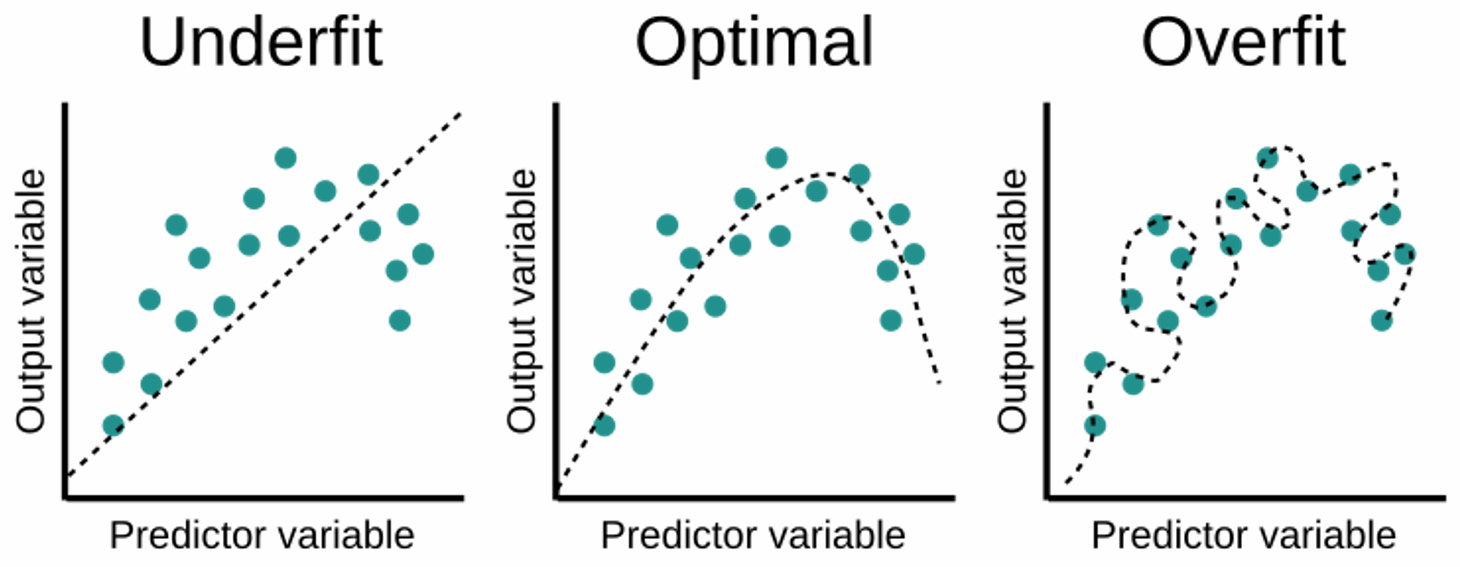
\includegraphics[width=0.75\paperwidth]{img/overfit_underfit.PNG}}
  \hspace*{15pt}\hbox{\scriptsize Source:\thinspace{\scriptsize\itshape towardsdatascience}}
\end{frame}


\begin{frame}
  \frametitle{Underfit, Optimal, Overfit and Model Complexity}
  \makebox[\linewidth]{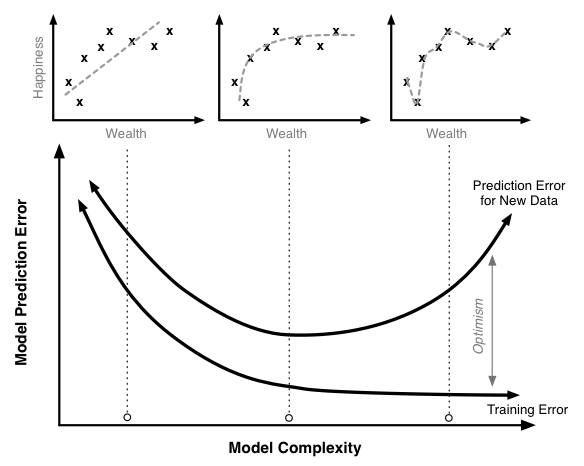
\includegraphics[width=0.55\paperwidth]{img/prediction_error_complexity.png}}
  \hspace*{15pt}\hbox{\scriptsize Source:\thinspace{\scriptsize\itshape Scott Fortmann-Roe}}
\end{frame}



\subsection{Out of Sample Concept}

\begin{frame}
  \frametitle{Out of Sample Concept}
  \makebox[\linewidth]{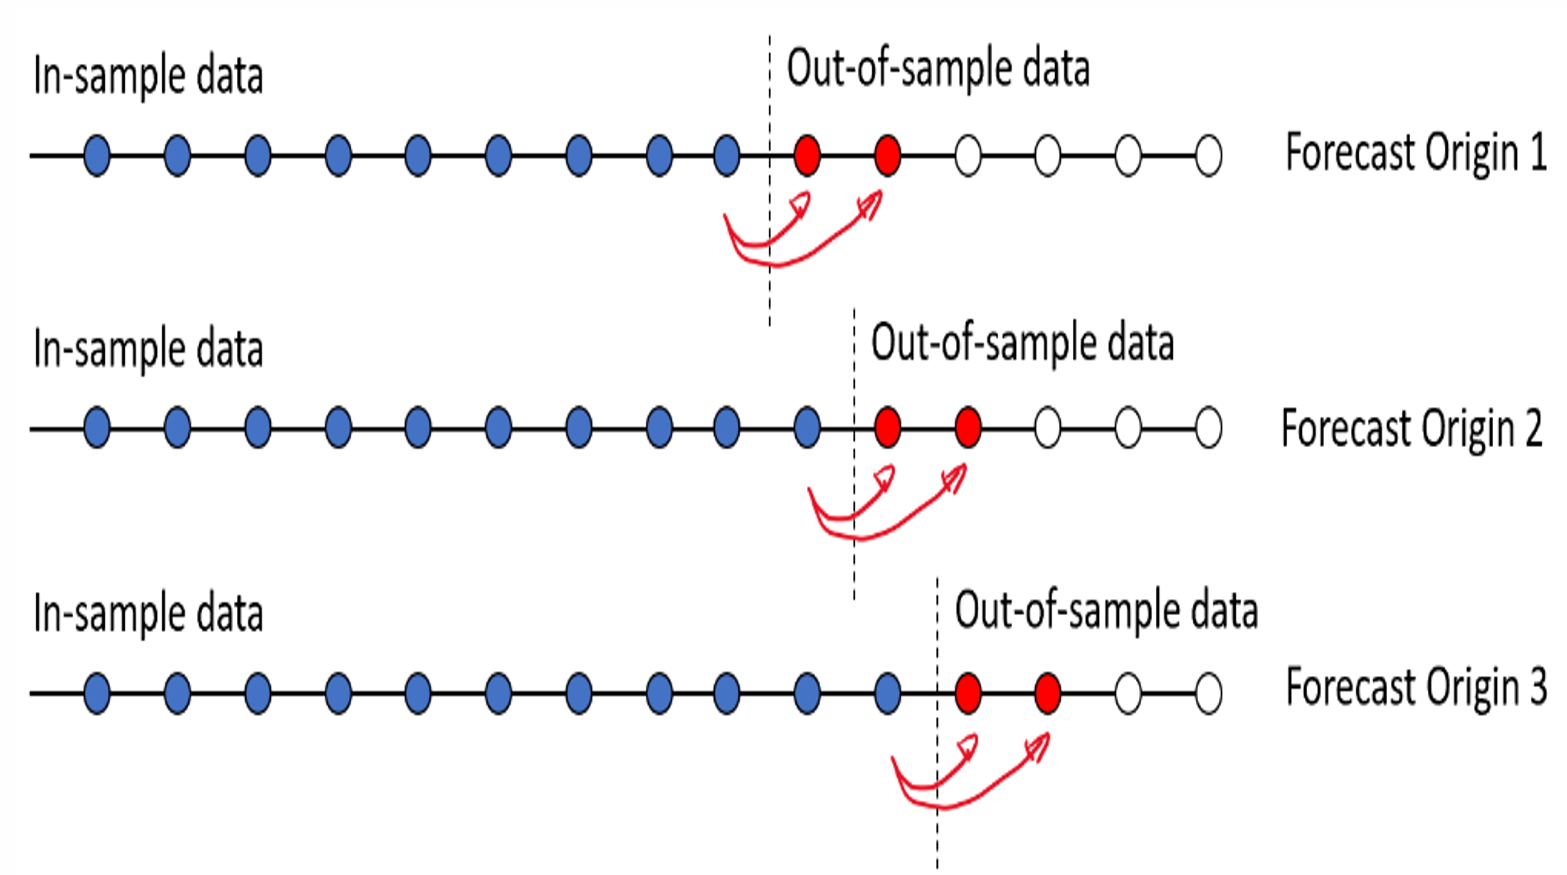
\includegraphics[width=0.75\paperwidth]{img/out_of_sample_concept.PNG}}
  \hspace*{15pt}\hbox{\scriptsize Source:\thinspace{\scriptsize\itshape Author}}
\end{frame}

\begin{frame}
  \frametitle{Out of Sample Example: Overfit}
  \makebox[\linewidth]{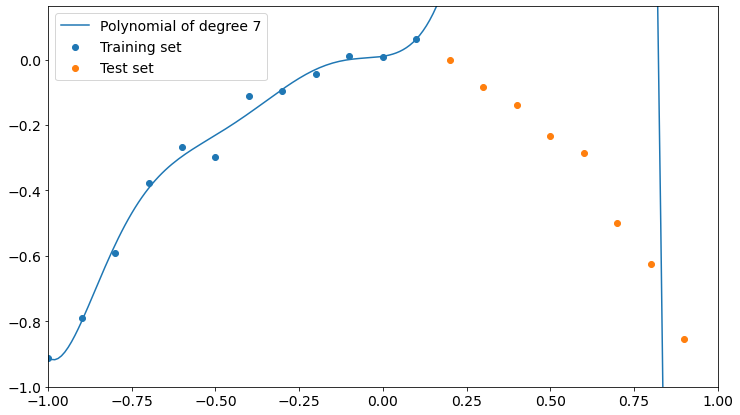
\includegraphics[width=0.85\paperwidth]{img/overfit_poly_7.png}}
  \hspace*{15pt}\hbox{\scriptsize Source:\thinspace{\scriptsize\itshape towardsdatascience.com/an-example-of-overfitting-and-how-to-avoid-it}}
\end{frame}


\begin{frame}
  \frametitle{Out of Sample Example: Correct Fit}
  \makebox[\linewidth]{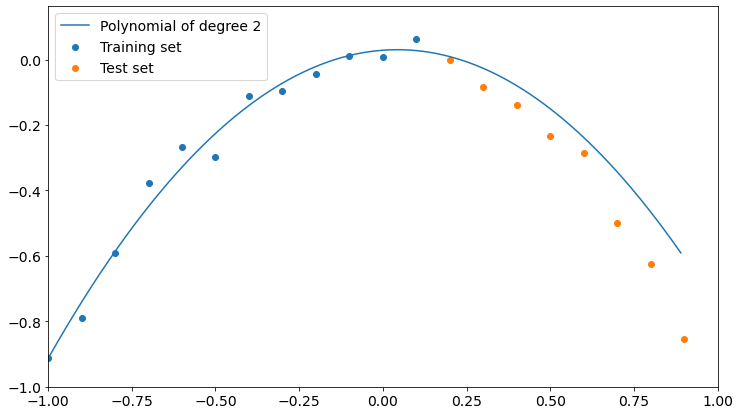
\includegraphics[width=0.85\paperwidth]{img/fit_poly_2.png}}
  \hspace*{15pt}\hbox{\scriptsize Source:\thinspace{\scriptsize\itshape towardsdatascience.com/an-example-of-overfitting-and-how-to-avoid-it}}
\end{frame}
  

\subsection{Cross-Validation}
\begin{frame}
  \frametitle{Time Series Cross-Validation}
     \makebox[\linewidth]{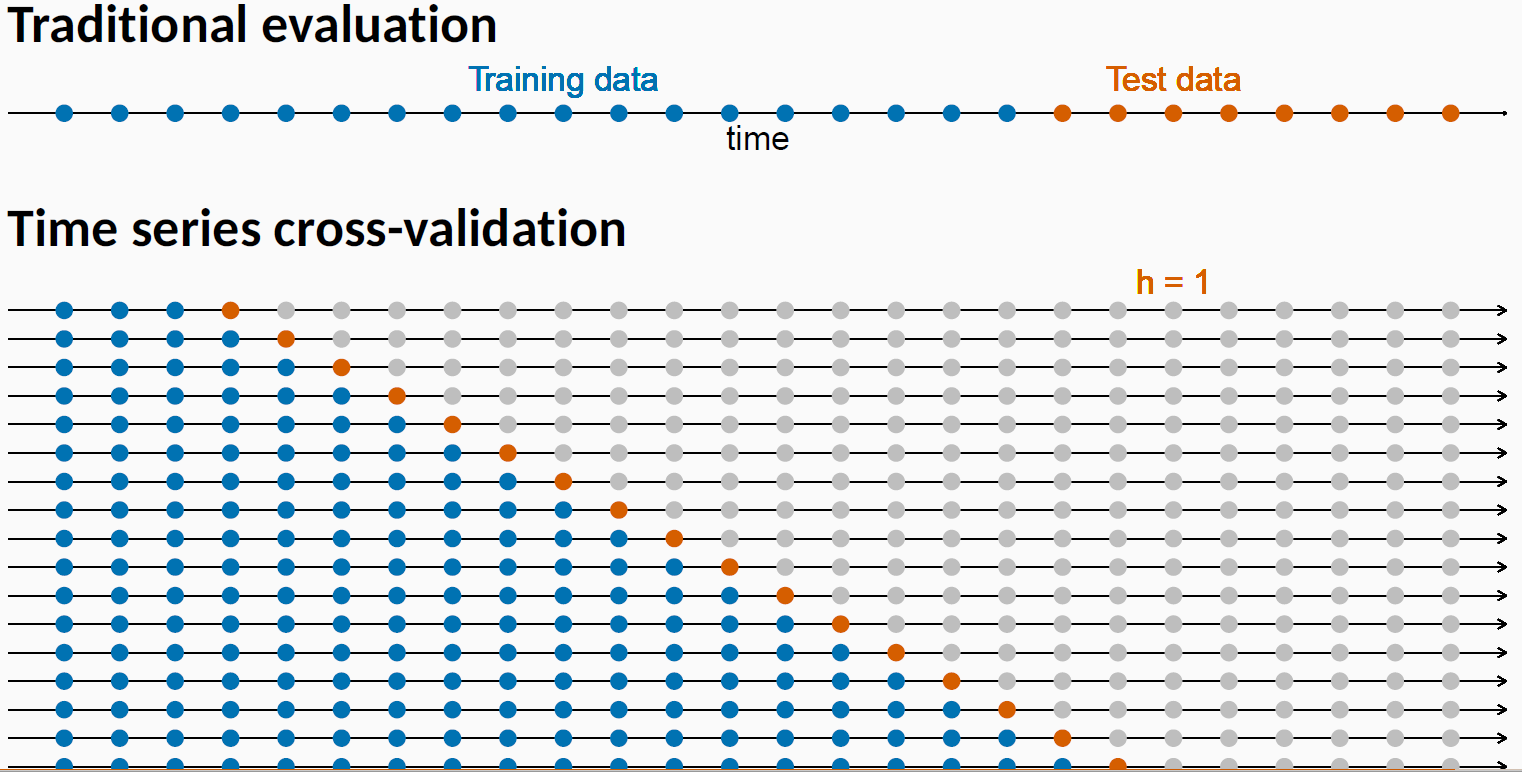
\includegraphics[width=0.95\paperwidth]{img/time_series_cv_1.PNG}}  
  \end{frame}

\begin{frame}
  \frametitle{Time Series Cross-Validation}
     \makebox[\linewidth]{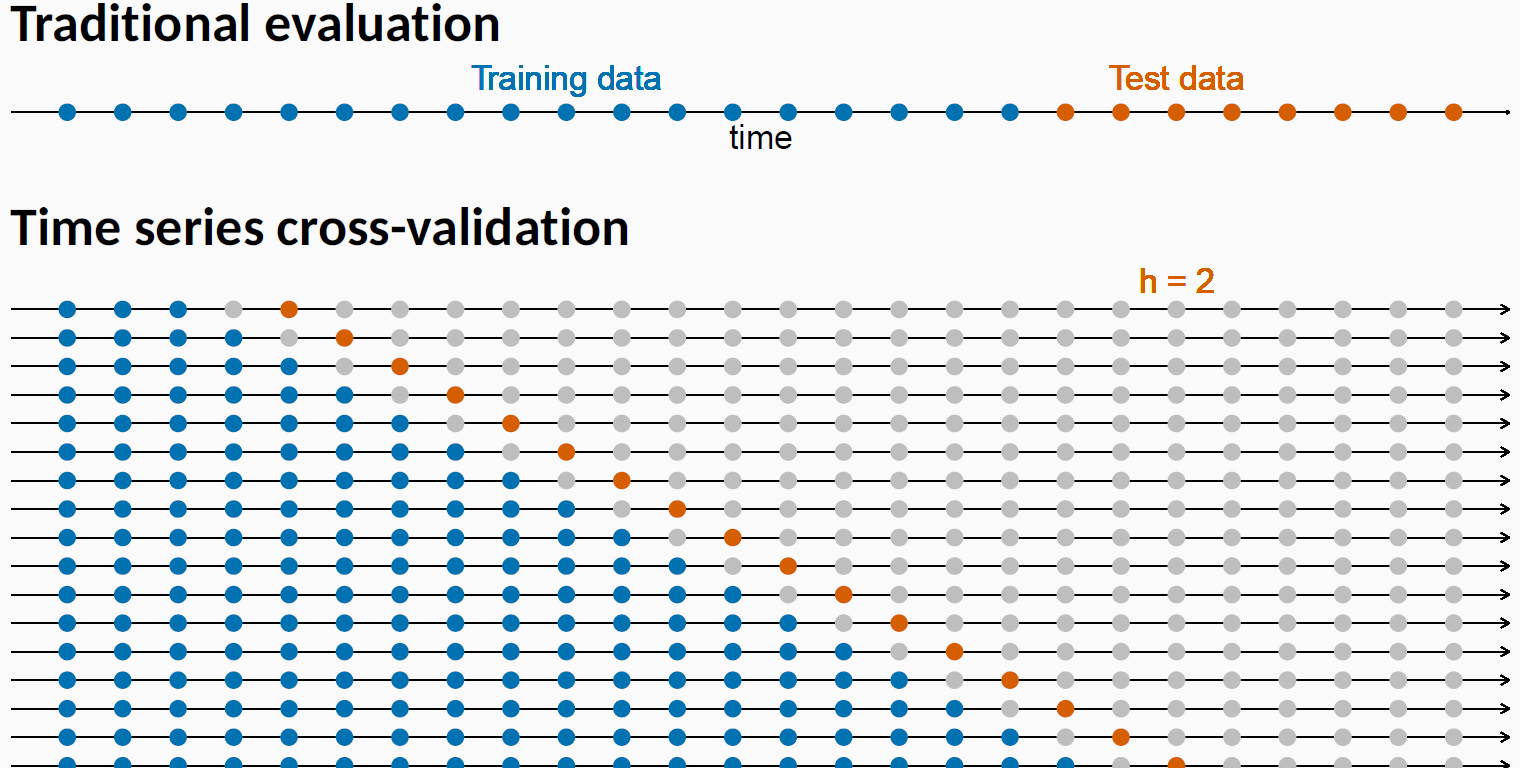
\includegraphics[width=0.95\paperwidth]{img/time_series_cv_2.PNG}}  
  \end{frame}

\begin{frame}
  \frametitle{Time Series Cross-Validation}
     \makebox[\linewidth]{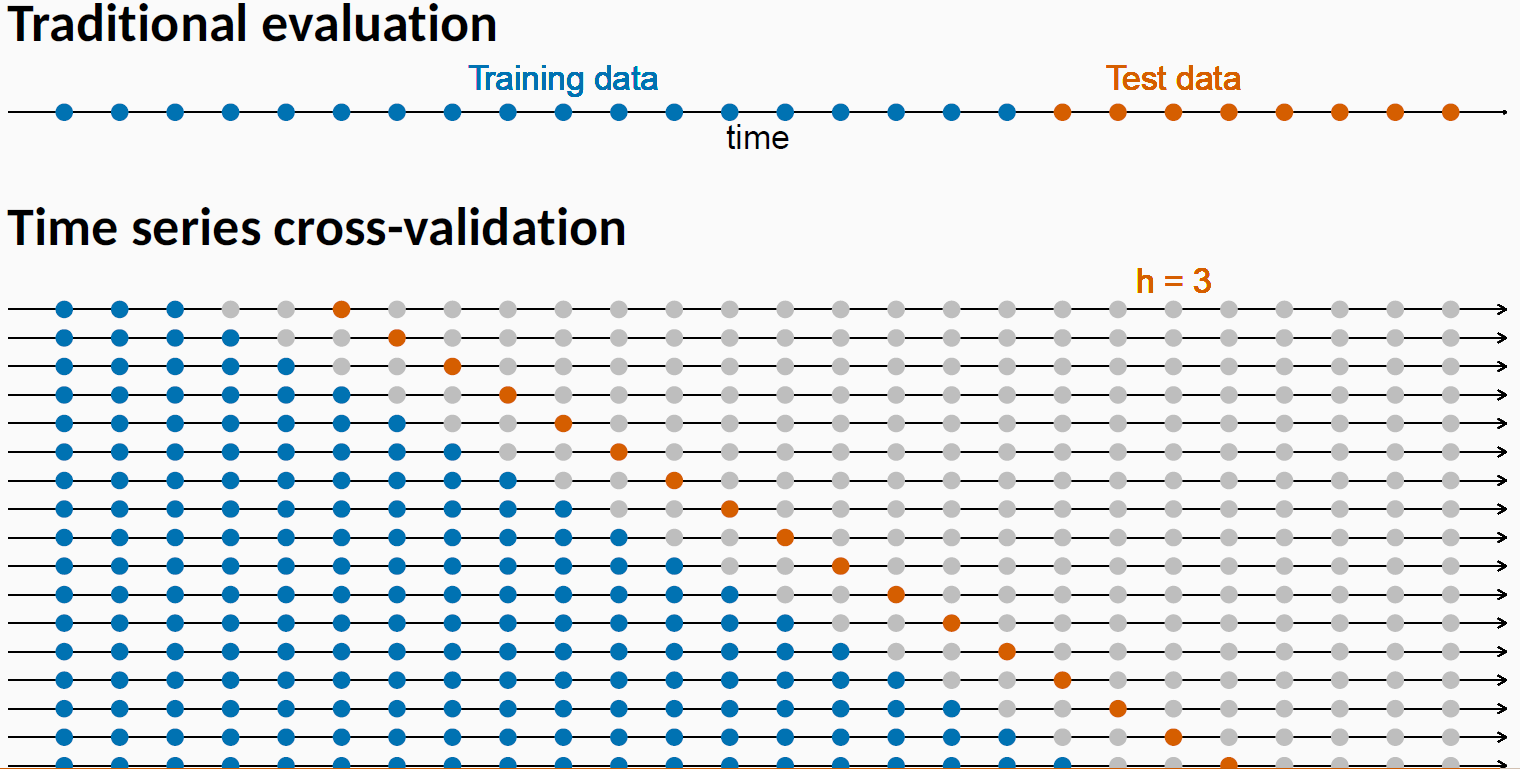
\includegraphics[width=0.95\paperwidth]{img/time_series_cv_3.PNG}}  
  \end{frame}

\begin{frame}
  \frametitle{Time Series Cross-Validation}
     \makebox[\linewidth]{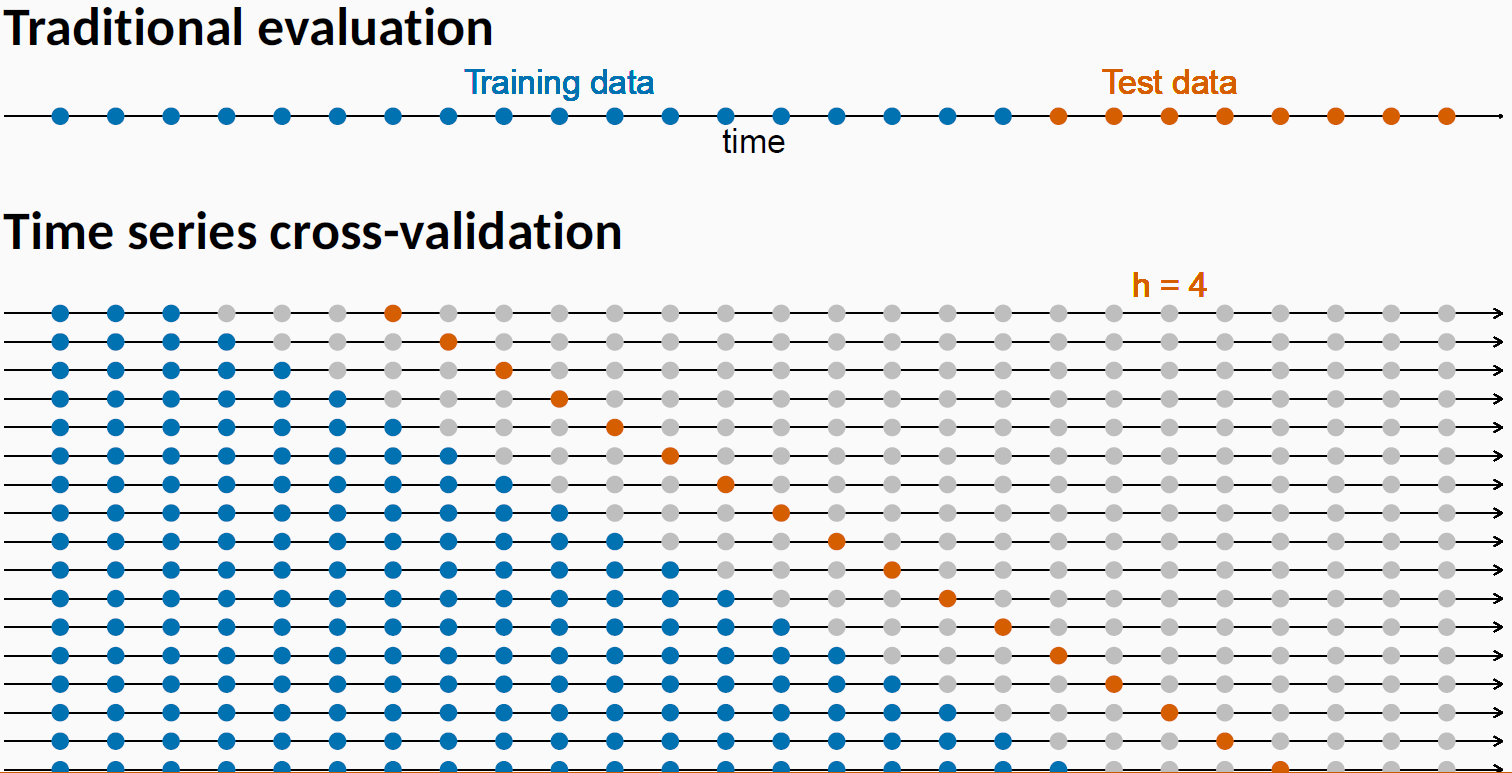
\includegraphics[width=0.95\paperwidth]{img/time_series_cv_4.PNG}}  
  \end{frame}

\begin{frame}
  \frametitle{Time Series Cross-Validation}
     \makebox[\linewidth]{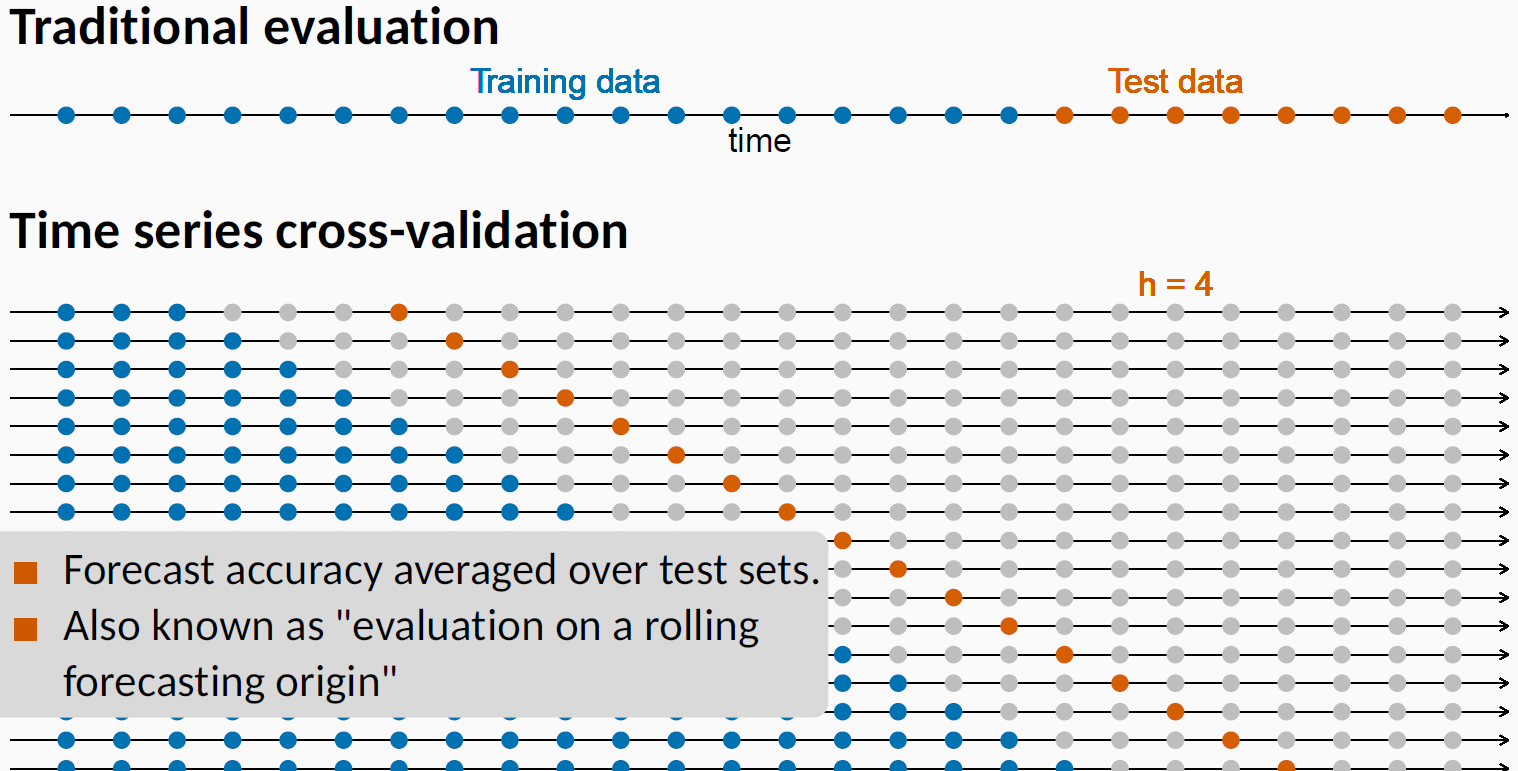
\includegraphics[width=0.95\paperwidth]{img/time_series_cv_5.PNG}}  
  \end{frame}


\section{Point-Forecasting Evaluation}


\begin{frame}
  \frametitle{Forecast Errors}
  \begin{wideitemize}
    \item Evaluating point forecasts are relatively straightforward
    \item Ex-post (after the realization happened), we observe:
      \begin{itemize}
      \item The true value $y_{T+h}$ that has been realized 
      \item The expected value $\hat{y_{T+h}}$ that has been generated before, in time $t$
      \end{itemize}
    \end{wideitemize}
      
  \begin{block}{Definition: Forecast Errors}
    A forecast error is the ex-post difference between an observed value and its forecast
    \begin{equation*}
      e_{T+h} = y_{T+h} - \hat{y}_{T+h}|Y_T, \dots, Y_1
    \end{equation*}
  \end{block}

  \begin{itemize}
  \item Forecast evaluation metrics represent different variations on how to summarize the $e_{T+h}$
    \begin{itemize}
    \item Are the forecast errors small on average? 
    \item Have we observed infrequent but large forecast errors (outliers)?
    \item Are the forecast errors evenly distributed across the distribution of $y$? etc.
    \end{itemize}
    
  \end{itemize}

\end{frame}


\begin{frame}{Forecast Errors with Train/Test Sets}

  \begin{alertblock}{Out of Sample}
    Measuring \textbf{accuracy} should be done out of sample. In-sample metrics inform on the how well the model \textbf{fits} the data
  \end{alertblock}
  
\begin{wideitemize}
    \item The conditional set $Y_T, \dots, Y_1$ should only be taken from the training dataset
    \item The true value $y_{T+h}$ is taken from the test set
    \item Unlike residuals, forecast errors on the test involve multi-step forecasts
    \item These are the \textbf{true} forecast error, as the test data is not used to compute $\hat{y}_{T+h}$
  \end{wideitemize}
  
\end{frame}

\begin{frame}
  \frametitle{Example: Forecasting Beer Production}
     \makebox[\linewidth]{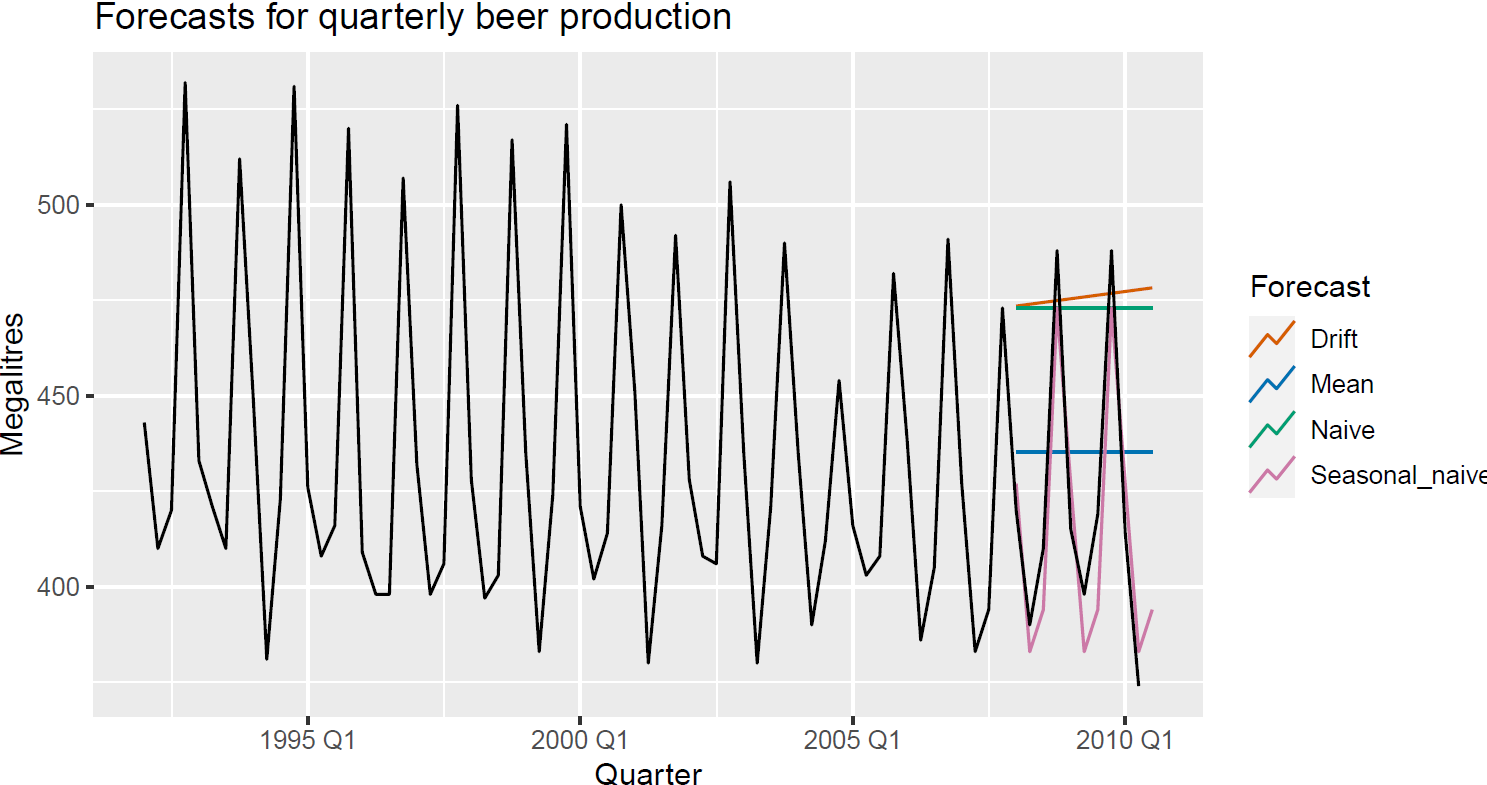
\includegraphics[width=0.95\paperwidth]{img/beer_forecast.PNG}}  
\end{frame}

\begin{frame}{Measures of Forecast Accuracy}

  \begin{alertblock}{Main Metrics}
    \begin{wideitemize}
    \item \textbf{MAE}: mean absolute errors $\frac{1}{S}\sum_{s \in S} |e_{s, T+h}|$
    \item \textbf{MSE}: mean squared errors $\frac{1}{S}\sum_{s \in S} (e_{s, T+h})^2$
    \item \textbf{MAPE}: mean absolute percentage errors $\frac{1}{S}100*\sum_{s \in S} \frac{|e_{s, T+h}|}{|y_{s, t+h}|}$
    \item \textbf{RMSE}: root mean squared errors: $\sqrt{\frac{1}{S}\sum_{s \in S} (e_{s, T+h})^2}$
    \end{wideitemize}
  \end{alertblock}

  With:\\
  
  \begin{itemize}
  \item $y_{T+h}$: T+h observation, h being the horizon (h = 1, 2, ..., H)
  \item $\hat{y}_{T+h|T}$: the forecast based on data up to time $T$
  \item $e_{T+h} = y_{T+h} - \hat{y}_{T+h|T}$: The forecast errors
  \item $S$ is the testing sample
  \end{itemize}
\end{frame}

\begin{frame}{Scaling}  
  \begin{wideitemize}
  \item MAE, MSE and RMSE are all \textbf{scale dependent}
  \item MAPE is scale independent but is only sensible if $y_t >> 0 \qquad \forall \ t$
  \item \textbf{Most commonly used: Time Cross-Validation with the lowest RMSE}
  \end{wideitemize}  
\end{frame}

    \begin{frame}
      \frametitle{Nemenyi Test}

      \begin{wideitemize}
        \item We can rank the model by RMSE (or another metric), but are the RMSE significantly different? 
        \item Maybe Model 1 can have a lower RMSE than Model 2, but the difference in RMSE is non-significant
        \item In which case, we could pool the two models together
        \item Use a non-parametric test to test the hypothesis of equal RMSE, with the test statistic:
          \begin{equation*}
            r_{\alpha, K, N} \approx \frac{q_{\alpha, K}}{\sqrt{2}} \sqrt{\frac{K (K+1)}{6N}}
          \end{equation*}
      \end{wideitemize}      
    \end{frame}

    \begin{frame}
      \frametitle{Nemenyi Test in Practice}
  \makebox[\linewidth]{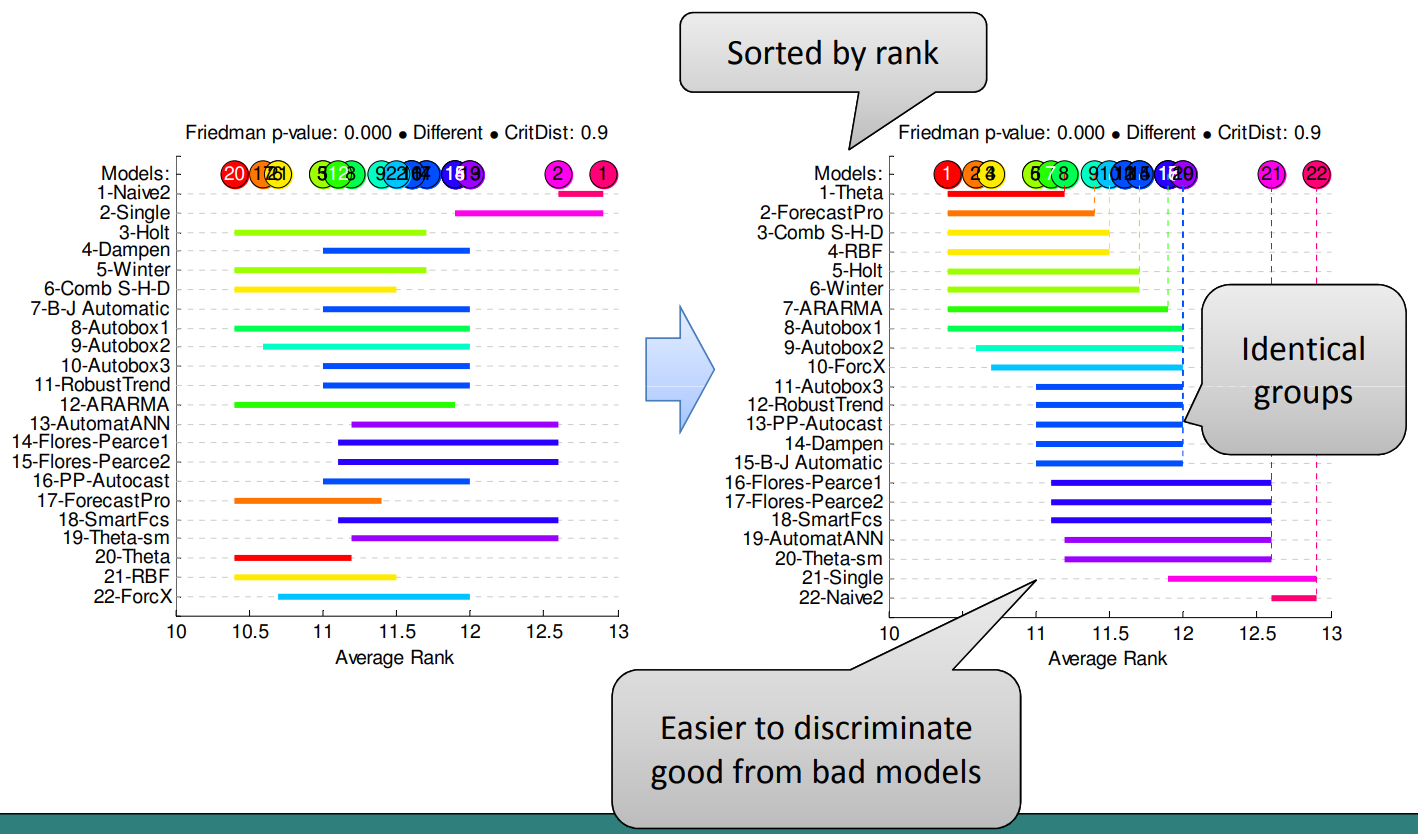
\includegraphics[width=0.85\paperwidth]{img/nemenyi_test.PNG}}
  \hspace*{15pt}\hbox{\scriptsize Source:\thinspace{\scriptsize\itshape Nikolaos Kourentzes}}      
    \end{frame}

    

\section{Density Forecast Evaluation}
    

\begin{frame}
  \frametitle{Challenges}
  \begin{wideitemize}
  \item At the difference of point forecasts, density forecasts are never observed
    \begin{itemize}
    \item We only observe \textbf{one} realization of the density
    \end{itemize}
  \item Hence, for evaluating the quality of the density forecasts, we need to use specific tools
   \item The \textbf{model specification}: is my model "neutral", not over-optimistic, not over-pessimistic?
      \begin{itemize}
      \item Use a \textbf{Probability Integral Transform (PIT) test}
      \end{itemize}      
    \item The \textbf{model performance}: attributing high \emph{ex-ante} performance to \emph{ex-post} realizations
      \begin{itemize}
      \item Use \textbf{logscores} and asymmetric logscores
      \end{itemize}
  \end{wideitemize}
\end{frame}


\begin{frame}
  \frametitle{Probability Integral Transform Test (PIT)}

    \begin{exampleblock}{Intuition}
      The forecasted quantiles from a correctly specified model should appear as frequently as their realizations. For instance, the true values should occur less than $10\%$ of the 10th quantile
        \begin{itemize}
        \item \textbf{Pessimistic model}: if the true values below the forecasted 10th percentile appear significantly more than 10\% of the time
        \item \textbf{Optimistic model}: if the true values below the forecasted 10th percentile appear significantly less than 10\% of the time
        \end{itemize}      
    \end{exampleblock}
        
  \begin{wideitemize}
    \item To quantify this approach, the PIT Test uses the concept of the probability integral transform
    \item A PIT is simply the evaluation of the cdf of a random variable ($F_x$) on its own realizations ($X_t$); the random variable $Y = F_X(X)$ should be uniformly distributed
    \end{wideitemize}
    
\end{frame}


\begin{frame}
  \frametitle{Probability Integral Transform}
  \makebox[\linewidth]{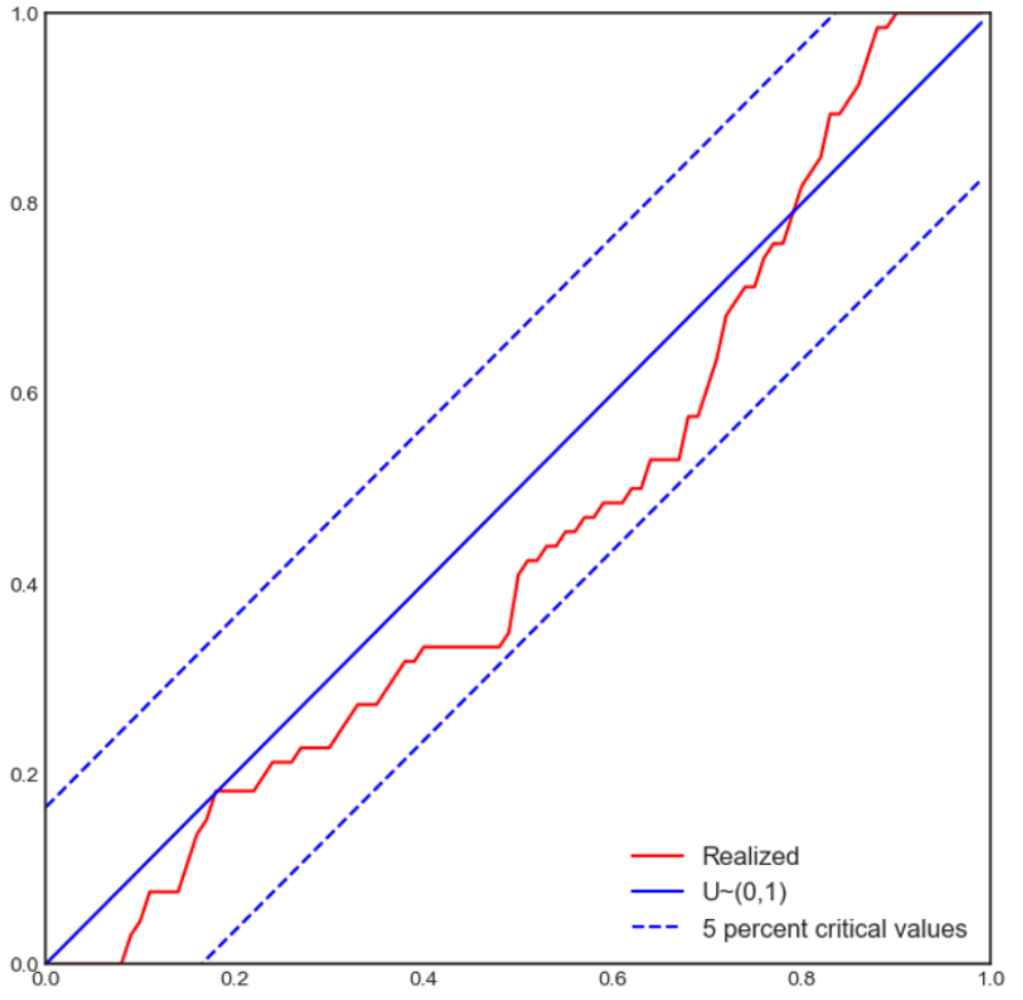
\includegraphics[height=0.7\paperheight]{img/pit_example.PNG}}
  \hspace*{15pt}\hbox{\scriptsize Source:\thinspace{\scriptsize\itshape Lafarguette (2019)}}        
\end{frame}


\begin{frame}
  \frametitle{Testing for the PIT}
  \begin{wideitemize}
    \item It is possible to test for the specification of the model looking at the distance between the theoretical line of 45 degrees
    \item However, there are always some randomness in the data: at which point the deviation becomes significant?
    \item Use the confidence interval computed by \href{https://ideas.repec.org/a/eee/econom/v208y2019i2p638-657.html}{\beamergotobutton{Rossi and Sekhposyan (2019)}}
      \begin{itemize}
      \item If the distribution crosses the confidence bands: the distribution is misspecified at this quantile
      \end{itemize}    
  \end{wideitemize}
\end{frame}


\begin{frame}
  \frametitle{Scoring Tests}
  \begin{wideitemize}
  \item PIT test answers the question: "is my model well specified"? 
  \item But it doesn't inform about the performance. If two models are well specified, how can we distinguish between them?
  \item Idea: score them based on their \emph{ex-post} performance of their \emph{ex-ante} forecasts
  \end{wideitemize}

  \begin{exampleblock}{Intuition}
    \begin{itemize}
    \item Idea: what was the \emph{ex-ante} probability of the \emph{ex-post} realization?
    \item Scores are usually taken in log-form: $S\left[\hat{f}_t(y_{t+h})\right] = \text{log}\left(\hat{f}_t(y_{t+h})\right)$
    \end{itemize}
  \end{exampleblock}
  
\end{frame}

\begin{frame}
  \frametitle{Ex-Ante Probability and Ex-Post Realizations }

  \makebox[\linewidth]{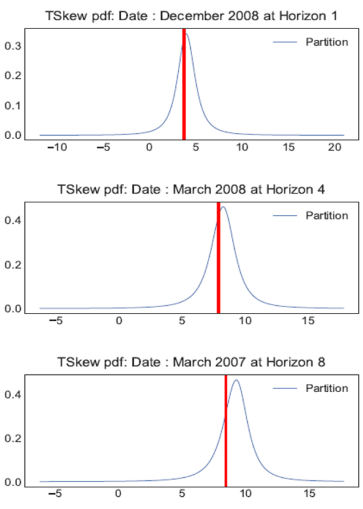
\includegraphics[height=0.65\paperheight]{img/logscores_overtime.PNG}}
  \hspace*{15pt}\hbox{\scriptsize Source:\thinspace{\scriptsize\itshape Lafarguette (2019)}}        
  
\end{frame}


\begin{frame}
  \frametitle{Tests for Equal Predictive Ability using Logscores}
  \begin{wideitemize}
    \item A logscore is a relative metric, for a single model, it doesn't inform (at the difference of PIT tests)
    \item However, the difference of logscores between models informs whether a model performs better than another one and should be preferred
    \item Need to assess whether the difference is significant if we want to test a model $\hat{f}$ against another one $\hat{g}$
    \item $d^{*}_{t+h} = \text{log}\left(\hat{f}_t(y_{t+h})\right) - \text{log}\left(\hat{g}_t(y_{t+h} \right) \qquad \qquad \bar{d^*}_{m, n} = \frac{1}{n} \sum_{t=m}^{T-1} d^{*}_{t+1}$
    \item Use the test of equal predictive ability via a Diebold-Mariano metric (1995)
      \begin{equation*}
        t_{m,n} = \frac{\bar{d^*}_{m, n}}{\sqrt{\hat{\sigma}^2_{m,n}/n}} \xrightarrow[n]{d} \mathcal{N}(0, 1)
      \end{equation*}
  \end{wideitemize}
\end{frame}


\begin{frame}
  \frametitle{Asymmetric Logscores}
  \begin{wideitemize}
    \item The simple difference provides information about how models performs "on average"
    \item However, density forecasts are especially useful to inform about risks 
    \item Hence, it makes sense to use \textbf{asymmetric logscores} to \textbf{test the performance in certain parts of the forecasted distribution}, especially on the tails
      \begin{equation*}
        \begin{split}
          S^{A}(\hat{f}_t, y_{t+1}) = & \mathbbm{1}\left(y_{t+1} \in A_t\right) \text{log}\hat{f}_t(y_{t+1}) \\
          & +  \mathbbm{1}\left(y_{t+1} \in A^c_t\right)\text{log}\left( \int_{A^c_t} \hat{f}_t(s) \text{d}s \right)
        \end{split}
      \end{equation*}
  \end{wideitemize}
\end{frame}

\begin{frame}
  \frametitle{Summary: Model Evaluation}
  \begin{wideitemize}
    \item To evaluate the performance of a model, it is crucial to evaluate its \textbf{out-of-sample performances} using \textbf{train and test samples}
    \item The evaluation of a \textbf{point forecast}, for instance the mean, can be evaluated from the \textbf{forecasting errors}, using different metrics: RMSE, MAE, MAPE, etc.
    \item The evaluation of a density is more complicated:
      \begin{itemize}
      \item To know if the density forecast is \textbf{properly specified}, use a \textbf{PIT test}
      \item To assess the \textbf{accuracy} of the model, use a \textbf{logscore} or an \textbf{asymmetric logscore}
      \item Note that other approaches, for instance based on \textbf{entropy}, exist: they try to minimize the amount of \textbf{information loss} between a density forecast and the true distribution
      \end{itemize}
  \end{wideitemize}

  
\end{frame}



\end{document}

%%% Local Variables:
%%% mode: latex
%%% TeX-master: t
%%% End:
